\documentclass[edeposit,tocnosub,noragright,centerchapter,fullpagesingle,12pt]{uiuc_csthesis21}

\makeatletter

\usepackage{setspace}  % Useful for single, 1.5, and double spacing
\usepackage[numbers, sort]{natbib}  % Useful for formatting reference section
\usepackage{url}  % Useful for URLs
%\usepackage{hyperref}  % Another package useful for URLs

\usepackage{lscape}  % Useful for wide tables or figures.
% Following command definition is from Stack Exchange: https://tex.stackexchange.com/questions/278113/single-landscape-page-with-page-number-at-the-bottom
% It adds *rotated* page numbers to the bottom of landscaped pages to meet the Graduate College standards (see page 7 here: https://grad.illinois.edu/files/pdfs/thesis-sample-chapter-straight-numbering.pdf)
\def\fillandplacepagenumber{
	\par
	\pagestyle{empty}
	\vbox to 0pt{\vss}
	\vfill
	\vbox to 0pt{
		\baselineskip 0pt
		\hbox to \linewidth{\hss}
		\baselineskip\footskip
		\hbox to \linewidth{\hfil\thepage\hfil}\vss
	}
}

%%%%%%%%%%%%%%%%%%%%%%%%%%%%%%%%%%%%%%%%%%%%%%%%%%%%%%%%%%%%%%%%%%%%%%%%%%%%%%%
% FIGURE PACKAGES
%
\usepackage{graphicx}  % Please import figures that are *high resolution* PDFs
%\usepackage{epsfig}   % or EPS files
\usepackage{caption}
%\usepackage{subfigure}  % Useful for subfigures
%\usepackage{subcaption}  % Useful for captioning subfigures

%\usepackage[utf8]{inputenc}
%\usepackage[inference]{semantic}
%\usepackage[english]{babel}
%\usepackage{csquotes}
%\usepackage{pifont}
%\usepackage{stmaryrd}
%\usepackage{microtype}
%\usepackage{amsmath,amsthm,amssymb}
%\usepackage[bookmarksdepth=3,linktoc=all,colorlinks=true,urlcolor=blue,linkcolor=blue,citecolor=blue]{hyperref}
%%\usepackage[style=ieee]{biblatex}
\usepackage[inline]{enumitem}
%\usepackage{dirtytalk}
%\usepackage{graphicx}
%\usepackage{wrapfig}
%\usepackage{subcaption}
%\usepackage{listings}
%\usepackage{xcolor}
%\usepackage{longtable}
%\usepackage{tabularx}
\usepackage{mathtools}
%\usepackage{varwidth}
%\usepackage{proof}
%\usepackage[bottom]{footmisc}
%\usepackage[bbgreekl]{mathbbol}

%%%%%%%%%%%%%%%%%%%%%%%%%%%%%%%%%%%%%%%%%%%%%%%%%%%%%%%%%%%%%%%%%%%%%%%%%%%%%%%
% TABLE PACKAGES
%
\usepackage{booktabs}  % Useful for high quality tables (e.g., you can replace \hrule with \toprule, \midrule, and \bottomrule).
%\usepackage{multicol}
%\usepackage{multirow}
%%%%%%%%%%%%%%%%%%%%%%%%%%%%%%%%%%%%%%%%%%%%%%%%%%%%%%%%%%%%%%%%%%%%%%%%%%%%%%%
% MATH PACKAGES (Comment out this section if unnecessary for your dissertation)
%
\usepackage{amsfonts}
\usepackage{amsmath}
\usepackage{amssymb}
\usepackage{amstext}
\usepackage{amsthm}
\usepackage[capitalize]{cleveref}


%\DeclareSymbolFontAlphabet{\mathbbm}{bbold}
%\DeclareSymbolFontAlphabet{\mathbb}{AMSb}%

% Change numbering of definitions, lemmas, theorems, etc to meet the Graduate College standards
\theoremstyle{definition}
\newtheorem{definition}{Definition}[chapter]
\newtheorem{lemma}{Lemma}[chapter]
\newtheorem{theorem}{Theorem}[chapter]
\newtheorem{corollary}{Corollary}[chapter]
\newtheorem{conjecture}{Conjecture}[chapter]
\newtheorem{remark}{Remark}[chapter]

\renewcommand{\qedsymbol}{QED.}  % Change symbol at end of proofs to meet the Graduate College standard
%%%%%%%%%%%%%%%%%%%%%%%%%%%%%%%%%%%%%%%%%%%%%%%%%%%%%%%%%%%%%%%%%%%%%%%%%%%%%%%
% ALGORITHM AND CODE PACKAGES (Comment out this section if unnecessary for your dissertation)
%
\usepackage{listings}  % Useful for formatting code blocks, see here for further information about formatting code: https://en.wikibooks.org/wiki/LaTeX/Source_Code_Listings
\usepackage[ruled]{algorithm2e}  % Useful for formatting algorithms (pseudocode)
\numberwithin{algocf}{chapter}     % Change numbering of algorithms to meet the Graduate College standards

%\definecolor{greybackground}{rgb}{0.95,0.95,0.92}
\definecolor{codegreen}{rgb}{0,0.6,0}
\definecolor{codegray}{rgb}{0.5,0.5,0.5}
\definecolor{codepurple}{rgb}{0.58,0,0.82}

% K lst definition
\lstdefinestyle{ksty}{
  keywordstyle=\color{magenta},
  basicstyle=\ttfamily\small,
  commentstyle=\color{codepurple},
  backgroundcolor=\color{greybackground},
  framerule=0pt
}
\lstdefinestyle{inlineksty}{
  basicstyle=\ttfamily\small
}
\lstdefinelanguage{k}{
  morekeywords={rule,configuration,=>,syntax,multiplicity,type,module,endmodule,import,imports, left,strict,seqstrict,bracket,structural,requires},
  morecomment=[l]{//},
  morecomment=[s]{/*}{*/}
}

% MediK lst definition
\lstdefinestyle{mediksty}{
  keywordstyle=\color{magenta},
  basicstyle=\ttfamily\small,
  commentstyle=\color{codepurple},
  backgroundcolor=\color{greybackground},
  framerule=0pt
}
\lstdefinestyle{inlinemediksty}{
  basicstyle=\ttfamily\small,
}
\lstdefinelanguage{medik}{
  morekeywords={either, or, machine, interface, vars, state, entry, on, do, goto, receives, ~>, =>},
  morecomment=[l]{//},
  morecomment=[s]{/*}{*/}
}

%Imp lst definition
\lstdefinestyle{impsty}{
  keywordstyle=\color{magenta},
  basicstyle=\ttfamily\small,
  backgroundcolor=\color{greybackground},
  commentstyle=\color{codepurple},
  framerule=0pt
}
\lstdefinelanguage{imp}{
  morekeywords={if, while, var}
  morecomment=[l]{//},
  morecomment=[s]{/*}{*/}
}

%\newcommand{\inlinemedik}[1]{\lstinline[style=inlinemediksty,language=medik]{#1}}
%\newcommand{\inlinek}[1]{\lstinline[style=inlineksty,language=k]{#1}}
%\newcommand{\inlineimp}[1]{\lstinline[style=impsty,language=imp]{#1}}
%\newcommand{\inlinekmath}[1]{\lstinline[mathescape,style=inlineksty,language=k,keepspaces]!#1!}
%\newcommand{\inlinemedikmath}[1]{\lstinline[mathescape,style=inlinemediksty,language=medik]!#1!}
%\newcommand{\inlinemedikimp}[1]{\lstinline[mathescape,style=inlineimpsty,language=imp]!#1!}
%\lstset{ literate={~}{{\raisebox{0.5ex}{\texttildelow}}}{1} }
%\lstset{captionpos=b,escapeinside={@}{@}}
%\providecommand*{\lstnumberautorefname}{Line}
%\def\boxit#1{%
%  \smash{\color{red}\fboxrule=1pt\relax\fboxsep=2pt\relax%
%  \llap{\rlap{\fbox{\vphantom{0}\makebox[#1]{}}}~}}\ignorespaces
%}
%
\graphicspath{{./figures}}
\newcommand{\frontend}{\emph{frontend}}
\newcommand{\BPG}{BPG}
\newcommand{\BPGs}{BPGs}
\newcommand{\CGS}{CGS}
\newcommand{\CGSs}{CGSs}
\newcommand{\HCP}{HCP}
\newcommand{\HCPs}{HCPs}
\newcommand{\ED}{ED}
\newcommand{\EDs}{EDs}
\newcommand{\CDSS}{CDSS}
\newcommand{\CDSSs}{CDSSs}
\newcommand{\BPGLogic}{knowledge-base}
\newcommand{\K}{\mathbb{K}}
\newcommand{\MediK}{\text{Medi}\K{}}
\newcommand{\FSM}{\emph{FSM}}
\newcommand{\FSMs}{\emph{FSMs}}
\newcommand{\Var}{\text{Var}}
\newcommand{\LHS}{\emph{\text{LHS}}}
\newcommand{\RHS}{\emph{\text{RHS}}}
\renewcommand{\phi}{\varphi}
\newcommand{\GUI}{GUI}
\newcommand{\UI}{UI}
\newcommand{\UIs}{UIs}
\newcommand{\GUIs}{GUIs}
\newcommand{\PME}{PME}
\newcommand{\PMEs}{PMEs}
\newcommand{\CIG}{CIG}
\newcommand{\CIGs}{CIGs}
\newcommand{\EHRs}{EHRs}
\newcommand{\ACLS}{ACLS}
\newcommand{\CPR}{CPR}
\newcommand{\CISs}{CISs}
\newcommand{\RTSs}{RTSs}
\newcommand{\ASMs}{ASMs}
\newcommand{\DSL}{\text{DSL}}
\newcommand{\DSLs}{\text{DSLs}}
\newcommand{\IT}{IT}
\newcommand{\EHR}{EHR}
\newcommand{\ONC}{ONC}
\newcommand{\NAM}{NAM}
\newcommand{\BNF}{BNF}
\newcommand{\MLM}{\text{MLM}}
\newcommand{\MLMs}{\text{MLMs}}
\newcommand{\GLIF}{\text{GLIF}}
\newcommand{\GEODECM}{\text{GEODE-CM}}
\newcommand{\PCAPE}{\text{P-CAPE}}
\newcommand{\DEGEL}{\text{DeGeL}}
\newcommand{\GLARE}{\text{GLARE}}
\newcommand{\GPROVE}{\text{GPROVE}}
\newcommand{\GOSPEL}{\text{GOSpeL}}
\newcommand{\GEE}{\text{GEE}}
\newcommand{\AAP}{\text{AAP}}
\newcommand{\NHS}{\text{NHS}}
\newcommand{\GP}{\text{GP}}
\newcommand{\GPs}{\text{GPs}}
\newcommand{\SAGE}{\text{SAGE}}
\newcommand{\MPS}{\text{MPS}}
\newcommand{\PC}{\text{PC}}
\newcommand{\PlanSet}{\text{PlanSet}}
\newcommand{\PatientSet}{\text{PatientSet}}
\newcommand{\ConditionSet}{\text{ConditionSet}}
\newcommand{\FinalStateSet}{\text{FinalStateSet}}
\newcommand{\Considered}{\text{Considered}}
\newcommand{\filter}{\text{filter}}
\newcommand{\possible}{\text{possible}}

% Convenience Commands
\newcommand{\cmark}{\text{\ding{51}}}
\newcommand{\xmark}{\text{\ding{55}}}
\newcommand{\greencheck}{{\color{green}\cmark}}
\newcommand{\redcross}{{\color{red}\xmark}}
\newcommand{\cancelcheck}{\bcancel{\cmark}}
\newcommand{\stress}[1]{\underline{\emph{#1}}}

% Scheduling Commands
\newcommand{\Machine}{\mathcal{M}}
\newcommand{\Instance}{\mathcal{I}}
\newcommand{\scheduled}{\textit{scheduled}}
\newcommand{\enabled}{\textit{enabled}}
\newcommand{\epoch}{\textit{epoch}}

% Logic-Related
\newcommand{\antecedent}[1]{\text{antecedent}\left(#1\right)}
\newcommand{\consequent}[1]{\text{consequent}\left(#1\right)}



%%%%%%%%%%%%%%%%%%%%%%%%%%%%%%%%%%%%%%%%%%%%%%%%%%%%%%%%%%%%%%%%%%%%%%%%%%%%%%%
% COVERPAGE
%

% Uncomment the appropriate one of the following four lines:
%\msthesis
\phdthesis
%\otherdoctorate[abbrev]{Title of Degree}
%\othermasters[abbrev]{Title of Degree}

\title{A Semantics-First Approach to Safe Guidelines-based Clinical Decision Support}
\author{Manasvi Saxena}
\department{Computer Science}
\degreeyear{2024}

% Advisor name is required for
% - doctoral students for the ProQuest abstract
% - master's students who do not have a master's committee
\advisor{Professor Grigore Ro\c{s}u}

% Uncomment the \committee command for
% - all doctoral students
% - master's students who have a master's committee
\committee{Professor Grigore Ro\c{s}u, Chair\\
        Professor Jose Meseguer \\
        Professor Lui Sha \\
        Doctor Serdar Tasiran, Amazon Web Services (AWS)} % etc.

\begin{document}

%%%%%%%%%%%%%%%%%%%%%%%%%%%%%%%%%%%%%%%%%%%%%%%%%%%%%%%%%%%%%%%%%%%%%%%%%%%%%%%
% COPYRIGHT
%
%\copyrightpage
%\blankpage

%%%%%%%%%%%%%%%%%%%%%%%%%%%%%%%%%%%%%%%%%%%%%%%%%%%%%%%%%%%%%%%%%%%%%%%%%%%%%%%
% TITLE
%
\maketitle

%\raggedright
\parindent 1em%

\frontmatter

%%%%%%%%%%%%%%%%%%%%%%%%%%%%%%%%%%%%%%%%%%%%%%%%%%%%%%%%%%%%%%%%%%%%%%%%%%%%%%%
% ABSTRACT
%
\begin{abstract}
  Preventable medical errors (PMEs), characterized by misdiagnosis or mistreatment,
  pose a significant challenge in healthcare.
  %According to a September 2023 report
  %by the President's Council on Science and Technology (PCAST) on patient safety,
  %a quarter of Medicare patients experience adverse outcomes during hospitalization,
  %of which 40\% were due to PMEs.
  In the United States, PMEs were estimated to have caused between
  44,000 and 98,000 deaths in 1997,
  rising to more than 250,000 in 2013. Additionally, the
  financial burden of PMEs to the U.S. economy in 2008 was estimated at \$19.5 billion.

  One strategy to reduce PMEs in medicine is through the use of
  clinical best practice guidelines (BPGs). BPGs are systematically developed,
  evidence-based statements published by medical institutions and associations
  that standardize diagnosis and treatment for various clinical scenarios.
  %Growing evidence indicates BPG-conformant treatment lowers the risk of preventable
  %medical errors.
 % However, following these guidelines in practice can be
 % challenging.
  %To assist with BPG-conformance, computerized
  %decision support systems that encode
  %medical knowledge in BPGs, and provide HCPs with relevant, situation-specific,
  %guideline-prescribed advice can be utilized.
  BPG-conformance has been linked with reduced rates of PMEs, but,
  following BPGs in practice can be challenging.
  Computerized Decision Support Systems (CDSSs) aim to improve conformance
  by encoding medical knowledge in BPGs and providing HCPs with
  situation-specific, guideline-conformant advice.
  Growing evidence suggests that
  effective CDSSs can reduce PMEs by boosting adherence to best practice guidelines.

  This work presents a semantics-first approach to implementing safe clinical
  decision support systems. By semantics-first,
  we mean that
  \begin{enumerate*}[label=\roman*]
    \item semantics of medical knowledge is
  accurately captured in the CDSS, and,
  \item the semantics of the programming language
    used to encode medical knowledge is formally defined.
  \end{enumerate*}
  At the core of our approach is \MediK{}: a novel domain specific language
  for expressing best practice guidelines that emphasizes comprehensibility
  to HCPs, enabling them to validate the accuracy of medical knowledge in its
  programs. \MediK{} has a complete, executable formal semantics in the \K{} Framework,
  from which all execution and analysis tools are derived in a
  correct-by-construction manner.

  To evaluate our approach, we collaborated with a major pediatric hospital
  to develop a complex real-world CDSS for the screening and management of
  Sepsis in pediatric cases, and validated that it satisfies desired safety properties.
  We outline how our approach improves upon the existing state-of-art,
  optimizations to address domain-specific needs of healthcare practitioners,
  and discuss challenges for future work.
\end{abstract}

%%%%%%%%%%%%%%%%%%%%%%%%%%%%%%%%%%%%%%%%%%%%%%%%%%%%%%%%%%%%%%%%%%%%%%%%%%%%%%%
% DEDICATION (Uncomment this section if desired)
%
\begin{dedication}
To my parents and my sister,
for their love and unconditional support,
and for always believing in me, even when challenges ensued.
\end{dedication}

%%%%%%%%%%%%%%%%%%%%%%%%%%%%%%%%%%%%%%%%%%%%%%%%%%%%%%%%%%%%%%%%%%%%%%%%%%%%%%%
% ACKNOWLEDGMENTS
%
\begin{acknowledgments}
While my journey at the University of Illinois has been long and challenging,
  I have been fortunate to have had the support of several wonderful people.

  First, I would like to thank my advisor, Prof. Grigore Ro\c{s}u,
  for his unwavering support and encouragement ever since I joined his research group as an undergraduate in the summer of 2014.

I am also extremely grateful to Prof. Lui Sha,
  with whom I have worked closely during the latter half of my PhD.
  His guidance, insights, and encouragement have been invaluable.
  I’d also like to thank him for his financial support, which enabled me to further develop my ideas.

I would like to express my sincere thanks to
  Dr. Serdar Tasiran for his mentorship during two summer internships at AWS’s S3 Automated Reasoning Group (S3-ARG),
  where I also had the opportunity to collaborate with Dr. Ankush Desai and Dr. Dongyun Jin,
  from whom I learned a great deal.
  I am also thankful to Serdar for impressing upon me the importance of
  effectively presenting ideas--a skill I have worked hard to improve based on his advice.

I am grateful to Prof. Jose Meseguer for his valuable insights
into implementing industrial-scale systems for use by non-experts in computer science.

I would also like to thank Prof. Rosu, Prof. Meseguer, Prof. Sha,
  and Dr. Tasiran for serving on my doctoral committee and for their time, expertise, and feedback.

I’d like to thank my labmates,
  both current and former, with whom I’ve had the pleasure of working with and learning from.
  Thank you, Daejun, Yi, Owolabi, Lucas, Xiaohong, Mircea, Nishant, Shuang, and Simon.
  A special shout-out goes to Nishant and Shuang for their companionship outside the lab,
  and to old friends Amulya, Neelabh, Rajiv, Dhruv, Balaji, and Aditya for always keeping me in the loop,
  even when I was too busy to respond.

I would like to extend my deepest gratitude to my family,
  both in the U.S. and in India.
I'd like to thank my uncle, aunt, and cousins, who always made sure I had a home away from home.
And to my parents and sister--thank you for the unconditional love, support, and unwavering belief in me, even during my moments of doubt.

\end{acknowledgments}

%%%%%%%%%%%%%%%%%%%%%%%%%%%%%%%%%%%%%%%%%%%%%%%%%%%%%%%%%%%%%%%%%%%%%%%%%%%%%%%
% TABLE OF CONTENTS
%
\tableofcontents

\mainmatter

%%%%%%%%%%%%%%%%%%%%%%%%%%%%%%%%%%%%%%%%%%%%%%%%%%%%%%%%%%%%%%%%%%%%%%%%%%%%%%%
% INSERT REAL CONTENT HERE
%

\chapter{Introduction}
\label{chp:intro}
%\section{Introduction}

Preventable Medical Errors (\PMEs{}) characterized by
incorrect intended treatment, or incorrect executions of intended
treatment present a significant challenge in Healthcare
\cite{RodziewiczStatsPearls18}. According to a seminal report on the subject
\cite{DonaldsonBook00}, in 1997,
between 44,000 and 98,000 deaths were estimated to have been caused by \PMEs{} in
the United States alone. A more recent study analyzed data from the eight-year
period between 2000 and 2008, and estimated that in 2013, the number of deaths
caused by \PMEs{} was more than 250,000, making \PMEs{} the third-leading
cause of death in the United States \cite{MakaryBMJ16}.
The adverse effects of \PMEs{} extend beyond patient outcomes.
One study estimated the financial burden of \PMEs{} to the United States to be
19.5 billion dollars in 2008 \cite{AndelJHCF12}. According to the authors of
\cite{RodziewiczStatsPearls18}, \PMEs{} caused psychological effects such
as anger and guilt in healthcare providers (\HCPs{}), adversely impacting their mental
health.

One strategy to mitigate \PMEs{} is to utilize evidence-based statements
published by hospital and medical associations that codify recommended
interventions for various clinical scenarios called Best Practice Guidelines (\BPGs{})
\cite{field1990clinical}. High quality guidelines are routinely updated to account for
 results from clinical trials and advances in medicine, and make the latest
 diagnosis and treatment information accessible to providers \cite{SteinbergNAP11}.

While \BPGs{} have the potential to reduce medical errors, their effectiveness hinges
on the adherence of healthcare providers to them.
For example, consider Advanced Cardiac Life Support (\ACLS{}): a \BPG{} published
by the American Heart Association (AHA) for management
of a life threatening condition called in-hospital cardiac arrest (IHCA) \cite{AHAGuidelineAdult, AHAGuidelinePed}. Studies suggest that management
of IHCA in 30\% of adult, and 17\% of pediatric cases deviates from the
AHA-prescribed \BPG, resulting in worse patient outcomes \cite{Ornato2012DeviationAdult,Wolfe2020DeviationPediatric,
Crowley2020DeviationAdult,Honarmand2018Adherence,Mcevoy2014Adherence}.

\begin{wrapfigure}{l}{0.5\textwidth}
  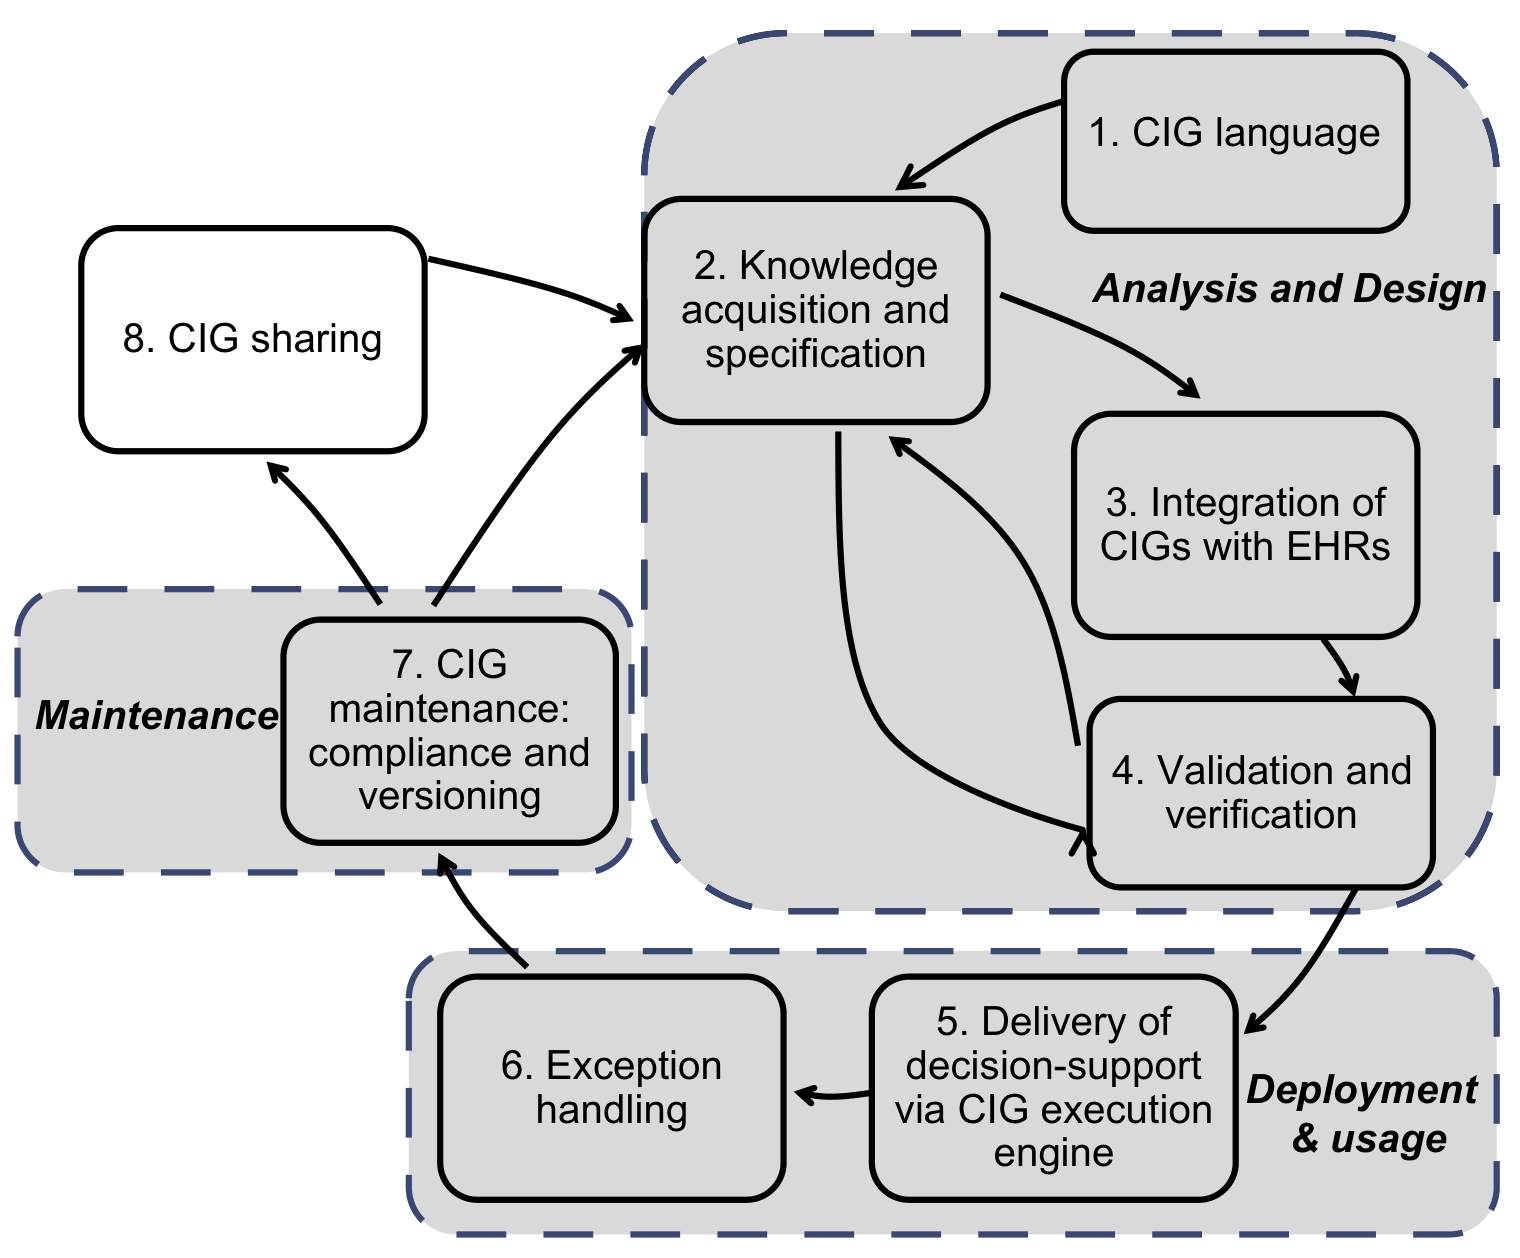
\includegraphics[width=\textwidth]{cpg-topics}
  \caption{\CDSSs{} Research Themes}\label{fig:cpg-research-topics}
\end{wrapfigure}

While \BPG{}-adherence is difficult to achieve in
practice \cite{RandJAMA99,DavisCMAJ97},
integrating \BPGs{} with existing patient care-flow,
and making them readily-accessible when required can improve adherence \cite{WoolfBMJ99}.
To this end, hospitals commission computerized Decision Support Systems (\CDSSs{})
that codify \BPGs{} and support \HCPs{} with situation-specific advice.
Such systems have been shown to improve \BPG{}-adherence \cite{GargJAMA06,KawamotoBMJ05}, and evidence from multi-center clinical trials
suggests that they reduce \PMEs{} \cite{BenettJAMIA16,SahotaJIS11}.
Thus, guideline-based \CDSSs{} are now considered imperative to the
future of medical decision making in general \cite{JamesNEJM01}.

While the potential of \CDSS{} has been recognized, wider adoption
is still hampered by significant challenges. \CDSSs{} are safety-critical -
bugs can have serious (sometimes life-threatening) consequences.
Thus, it's vital that:
\begin{enumerate*}[label=(\alph*)]
  \item the system is formally verified to satisfy desired correctness
    properties, and,
  \item \HCPs{} can trust the medical knowledge embedded in the system.
\end{enumerate*}
While research on \CDSSs{} has resulted in progress towards addressing
these challenges, more work is needed to realize their full potential.
We briefly provide an overview of existing research on \CDSSs{} to explain
both progress made and challenges remaining in context of \CDSSs{}.
In \cite{PelegJBI13}, the author provides a methodological review of
existing work on Computer Interpretable Guidelines (\CIGs{}): executable
formalizations of \BPGs{} used to construct \CDSSs{}.
Existing work is classified into one of eight themes spanning
the entire development cycle of a \CIG{}. The themes and relations between them
are shown in \figurename{} \ref{fig:cpg-research-topics}.

According to the author in \cite{PelegJBI13}, \CIGs{} are usually based on previously published non-executable
\BPGs{}. To develop a \CIG{}, a language is identified in (1). Teams of
software developers and clinicians then collaborate to express medical knowledge
in the \BPG{} in the identified language. In (3), the \CIG{}
is integrated with components such as a Graphical User
Interface (\GUI{}), Electronic Health Records (\EHRs{}) and external devices
(such as monitors for patient parameters) to obtain a \CDSS. Before adoption
in the real-world, it is imperative to ensure that the \CIG{} \emph{mirrors}
the underlying \BPG{}. This validation occurs by \emph{testing} the \CDSS{}
using execution capabilities of the modeling language from (1) in (5).
Additionally, formal verification may be used to establish other desired
properties hold. Inconsistencies identified in (5) are fixed through developer-clinician
collaboration in (2),  re-validation and
verification. While the aforementioned development cycle has resulted in several
effective \CDSSs{}, it has some limitations:

\paragraph{Gap between specification and implementation:}

To develop the \CIG{}, software developers rely on clinicians to interpret the
non-executable \BPG{} and communicate
the intended semantics to them. Thus, the non-executable \BPG{} serves as a functional specification for
the \CIG{}, i.e. the implementation. In such safety-critical systems, it is
imperative that the implementation, i.e. the \CIG{}, conforms to its
specification, i.e., the \BPG{}. To address this, the \CIG{} is tested by
putting the \CDSS{} through clinical simulations. But, while testing reduces
the risk of non-conformance, it does not completely eliminate it.

%\paragraph{Safe Modularity:}
%
%While developing \CDSSs{} is both complex and cost-intensive,
%the development effort can be reduced by sharing \CDSSs{} across hospitals \cite{PelegAMIA00}.
%But, even for the same \BPG{}, hospitals develop their own \CDSSs{} to address
%their needs, resulting in duplicated work.
%For instance, for the \ACLS{} \BPG{}, multiple \CDSSs{} have been developed by different
%different hospitals in a span of just six years years \cite{FullCodePro,PediAppRREST2020,
%PediAppRREST2021,GuidingPad2017,GuidingPad2019, GuidingPad2020,DST2014,DST2019,ROSCo2021,TeamScreen2019,Wu2017}.
%\CDSSs{} based on the same \BPG{} typically have the same \CIG{}, but may differ
%in their Graphical User Interfaces (\GUIs), or integration with external
%devices, to address hospital-specific needs.
%To enable safe sharing of knowledge, we need a mechanism that:
%\begin{enumerate*}[label=(\alph*)]
%  \item allows a stable, formally-verfied \CIG{} that is \emph{decoupled} from other
%    components, and,
%  \item supports hospital-specific customizations without compromising system
%    \emph{safety}.
%\end{enumerate*}


\paragraph{Formal semantics and analysis tools:}

Given the safety-critical nature of \CDSSs{}, it is vital for \CIG{} languages
to have complete formal semantics and formally-verified execution engines and
analysis tools. This need has already been recognized in existing literature
\cite{SuttonAMIA03, ShaharAMIA96}. It's also vital to ensure that
associated tools are kept up to date as the language evolves.

\paragraph{Holistic system safety:}

While the safety critical nature of \CDSSs{} neccessitates
\CIG{} languages to have comprehensive support for verification using
tools like model checkers and deductive verifiers, certain challenges
specific to \CDSSs{} require support beyond traditional techniques.

Actions performed by a \CDSS{} can either be \emph{programming-oriented}
or \emph{clinically-oriented} \cite{BoxwalaJBI04}. \emph{Programming-oriented}
actions are peformed by executing the \CIG{} itself. For example,
using patient parameters, or health records to make a reccomendation or diagnosis,
or to raise a warning. \emph{Clinically-oriented} actions on the other hand
are ones that involve a clinician. For example, in the case of \ACLS{},
the \CDSS{} recommends that Cardiopulmonary Resuscitation (\CPR{}) be performed
for a certain length of time. Such actions can only be performed by clinicians,
an the \CDSS{} assumes that the recommended action was indeed performed before
moving resuming guidance.

For correctness, both categories of actions must be completed
successfully. While traditional formal reasoning techniques can be employed
to establish correctness of \emph{programming-oriented} actions, the same
cannot be used to reason about \emph{clinically-oriented} ones.
Thus, a mechanism that allows some guarantees about clinically-oriented is
desirable.

This proposal aims to address these limitations comprehensively
using a \emph{semantics-first} approach.
By \emph{semantics-first}, we mean that \CIG{} language we
use to is formally defined, from which tools such as an interpreter, model checker,
and deductive verifier are derived in a \emph{correct-by-construction}
manner. At the core of our approach is new language Domain Specific Language (DSL)
for \CIGs{} called \MediK{}. By emphasizing \HCP{}-\emph{comprehensibility},
\MediK{} enables \HCPs{} to verify the semantic correctness of a \CIG{}.
\MediK{} provides a uniform way of modeling diverse external agents, enabling reasoning about
safety of the entire system.

\MediK{} has been used to implement a real-word \CDSS{} for screening and
mangement of pediatric sepsis, and establish said \CDSS{} satisfies desired
safety properties. To the best of our knowledge, it is the first system
for sepsis management with formal safety guarantees.

While \MediK{} presents a promising direction towards developing safe real-world
systems, realizing its full potential requires addressing the following research
challenges (RCs):

\paragraph{RC 1 (Design):} Is \MediK{}'s design conducive to expressing diverse \BPGs{}?

\BPGs{} can vary greatly by scope and purpose. For instance,
consider differences between the \BPGs{} for managing cardiac
arrest and sepsis. The \BPG{} for cardiac arrest can be
succinctly depicted by a single workflow. On the other hand, the \BPG{} for
screening and management of sepsis involves multiple workflows with complex
inter-workflow interactions.
This proposal seeks to answer whether \MediK{}'s
design can adequately accomodate diversity in \BPGs{}, without
compromising on readability. To this end, we plan to collaborate with
experts in medicine to ensure that the language meets their needs.
Note that the \emph{semantics-first} approach is particularly
well-suited for designing the language, as updates to the language
only require changes to the semantics. As tools are derived from the semantics,
they update automatically.

\paragraph{RC 2 (Ecosystem):} Does \MediK{} have a mature
set of tools that enable building safe \CDSSs{}?

\MediK{} has a complete executable formal semantics, from which
its tools are derived in a \emph{correct-by-construction} fashion.
But, as real-world \BPGs{} are complex, establishing appropriate safety and liveness properties using
said tools presents various challenges. The proposal seeks to build on
\MediK{}'s toolchain to support verification of desired safety and liveness
properties of large \BPGs{}.

While $\K$ derived tools enable execution and analysis of \MediK{} programs,
certain \BPG{}-specific requirements may not have direct $\K{}$ equivalents.
In such cases, this proposal seeks to develop new semantics-based tools within
the $\K{}$ ecosystem, that are vital in \MediK's context, but may also have
applications for other $\K$-based languages.
For instance, visual representations of \MediK{} programs can
significantly improve comprehensibility of \MediK{} programs to medical domain
experts. This proposal seeks to expand on techniques
such as semantics-based compilation that can be used to extract information such
as basic blocks from code to generate \emph{correct-by-construction} visual
representation of programs in any language.

\paragraph{RC 3 (Applications):} Can \MediK{} be used to build real-world
\CDSS{}? How can \MediK{} improve \CDSSs{} effectiveness?

This proposal
seeks to establish that our approach can be used to build systems with real
world applications. To this end, we plan to build \CDSSs{} that are
capable of consideration for clinical trials at hospitals. Note that we
intend to use clinical-trial worthiness as an indicator of the effectivenss
of \MediK{}, not the result of the trial itself.
Clinical-trial worth systems need to be integrated into existing hospital care-flow.
This involves handle hospital-specific variations, such as
diversity in data sources and health records. This proposal seeks to
develop the \MediK{} ecosystem to a point where it can be used to build
such systems.

This proposal also seeks to develop new \CDSS{} capabilities enabled by the
\emph{semantics-first} approach. In particular, our approach
enables the following capabilities:

\begin{itemize}
  \item \textbf{Guideline Adherence Proofs:} Execution of a
\MediK{} \BPG{} is simply a proof in Matching Logic (ML), the logic
underlying the $\K{}$ framework, using the semantic rules as axioms.
Said proofs can be checked by an external ML proof-checker.
In \MediK{}'s case, execution proofs can serve as evidence of adherence to best practices during treatment.
Moreoever, zero-knowledge proofs can allow hospitals to establish
conformance to best practices, without divulging sensitive information
such as \emph{patient data} or \emph{specific treatment}
  \item \textbf{Safe Incorporation of Artificial Intelligence (AI):}
Advances in AI have applications in medicine. AI-based components
can enable early detection and targed treatment of medical conditions.
However, integrating such systems \emph{safely} remains a challenge,
\emph{hallucinations} in AI-based systems can lead to serious consequences.
We seek to explore \emph{safe} incorporation of AI-based systems into cafe-flow using
a simplex-based approach, where recommendations from an AI-based component are
\emph{checked} against known best practices before they're enacted.
If the recommendation is determined to be unsafe, a fallback action is enacted
instead.
\end{itemize}


  % Inserts content from "introduction.tex" here

 NOTE 1: The Graduate College standards allow sections to be numbered by chapter number, section number, and subsection number. This means you can use the following commands within a chapter:
 \cite{RosuJLAP10}
 \section{}
% \subsection{}
% \paragraph{} (does not produce a number)
% In other words, do not use the command \subsubsection{} and beyond!

% NOTE 2: The Graduate College is picky about access white space, so you should attempt to minimize access whitespace when possible. For example, Latex will move a section header and subsequent paragraph onto the next page to avoid having a section header followed by a single line of text. In this case, you should use the command "\clearpage \noindent" at the end of the first line text in the paragraph to try to bump the header and one line of text back onto the previous page.

%\chapter{Conclusions}
%\label{chp:concl}
%\input{conclusions}  % Inserts content from "conclusions.tex" here

%%%%%%%%%%%%%%%%%%%%%%%%%%%%%%%%%%%%%%%%%%%%%%%%%%%%%%%%%%%%%%%%%%%%%%%%%%%%%%%
% BIBLIOGRAPHY
%
\bibliographystyle{IEEE_ECE}
\bibliography{references}  % Put references in BibTeX format in thesisrefs.bib.

%%%%%%%%%%%%%%%%%%%%%%%%%%%%%%%%%%%%%%%%%%%%%%%%%%%%%%%%%%%%%%%%%%%%%%%%%%%%%%%
% APPENDIX
%
% NOTE: Appendices go *after* the bibliography (see here: https://grad.illinois.edu/thesis/format). However, if appendices contain citations, then you may move the appendices *before* the bibliography section.
\appendix

%\chapter{Something}
%\label{apx:something}
%\input{appendix-something}  % inserts content from "appendix-name.tex"

\backmatter

\end{document}
\endinput
